\documentclass[11pt]{article}

\usepackage{fancyhdr}
\usepackage{enumerate}
\usepackage{comment}
\usepackage{tabularx}
\usepackage{booktabs}%make tables look better. 
\usepackage{colortbl}
\usepackage{enumitem}
\usepackage{amsmath}
\usepackage[table]{xcolor}
\usepackage[normalem]{ulem}
\usepackage[edges]{forest}
\usepackage{soul}
\usepackage{amssymb} 
\usepackage{graphicx}
\usepackage{subcaption}

\oddsidemargin0cm
\topmargin-2cm    
\textwidth16.5cm   
\textheight23.5cm  

\newcommand{\question}[2] {\vspace{.25in} \hrule\vspace{0.5em}
\noindent{\bf #1: #2} \vspace{0.5em}
\hrule \vspace{.10in}}

\newcommand\tab[1][1cm]{\hspace*{#1}}
\newcommand{\myname}{Adele Swecker}
\newcommand{\mycourse}{Gender Studies}
\newcommand{\myhwnum}{Final}

\setlength{\parindent}{0pt}
\setlength{\parskip}{5pt plus 1pt}
\setlength{\headheight}{13.59999pt}

\pagestyle{fancyplain}
\lhead{\fancyplain{}{\textbf{\myhwnum}}}      % Note the different brackets!
\rhead{\fancyplain{}{\myname}}
\chead{\fancyplain{}{\mycourse}}

\begin{document}

\thispagestyle{plain}
\begin{center}
  {\Large \mycourse\ \myhwnum} \\
  \myname
\end{center}

For my final project, I decided to convert our readings from the current pdfs into readable files 
so that I can compile and add all instance of keywords. I selected a few key words and outputed their 
occurences to showcase existing bias in our work. The counts are as accurate as I can make them but 
some words were lost in the translation of pdf to text.

\question{Word Counts including "the" for reference}

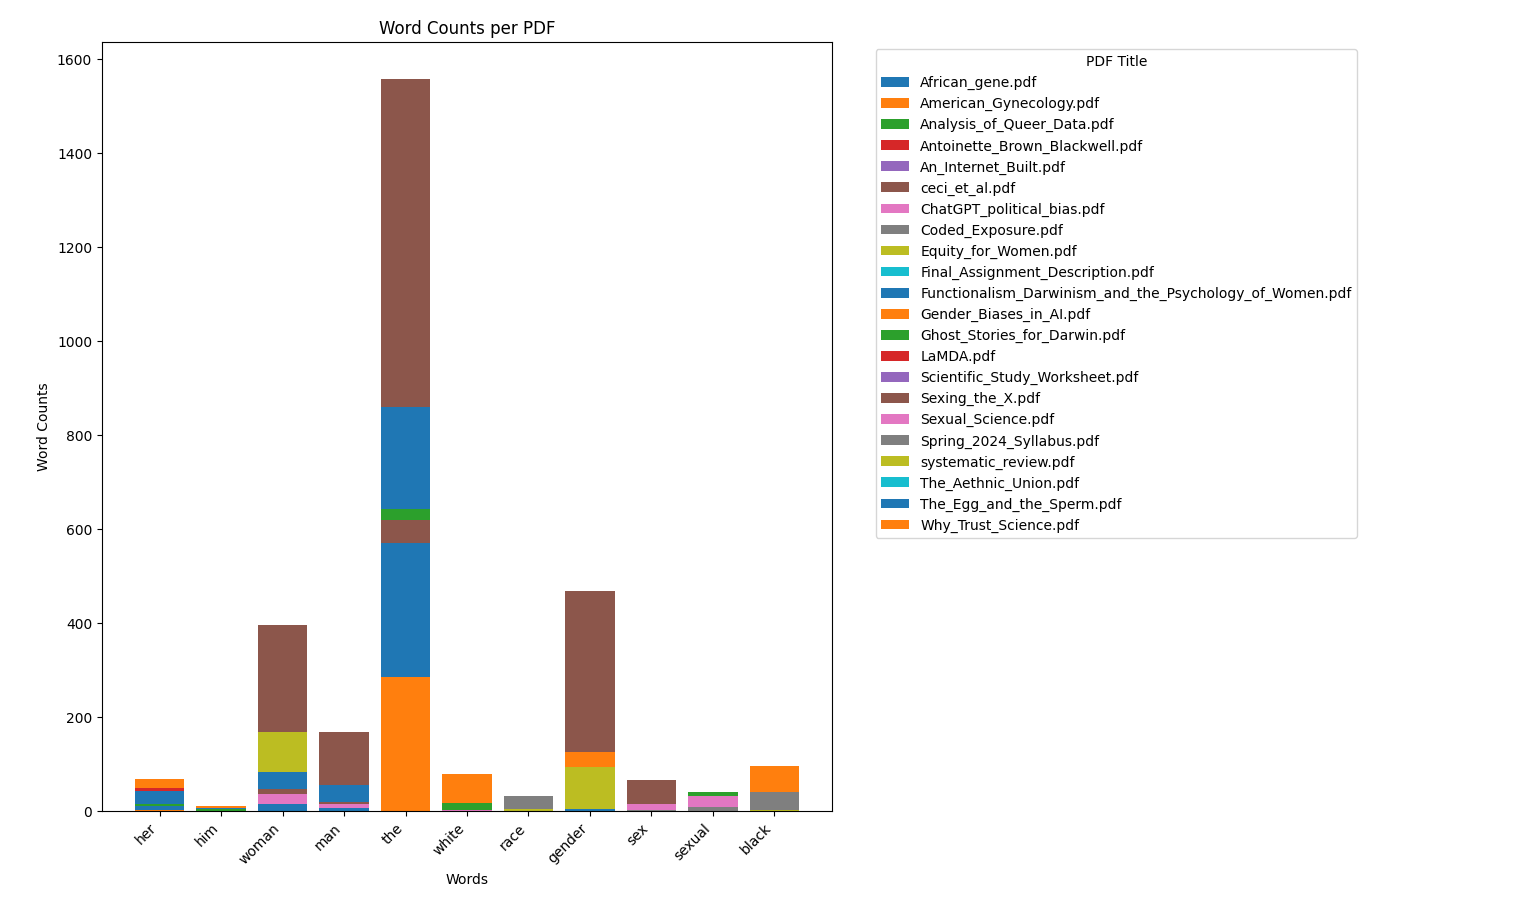
\includegraphics[width=\textwidth]{word counts including the.png}

\break

\question{Word Counts}

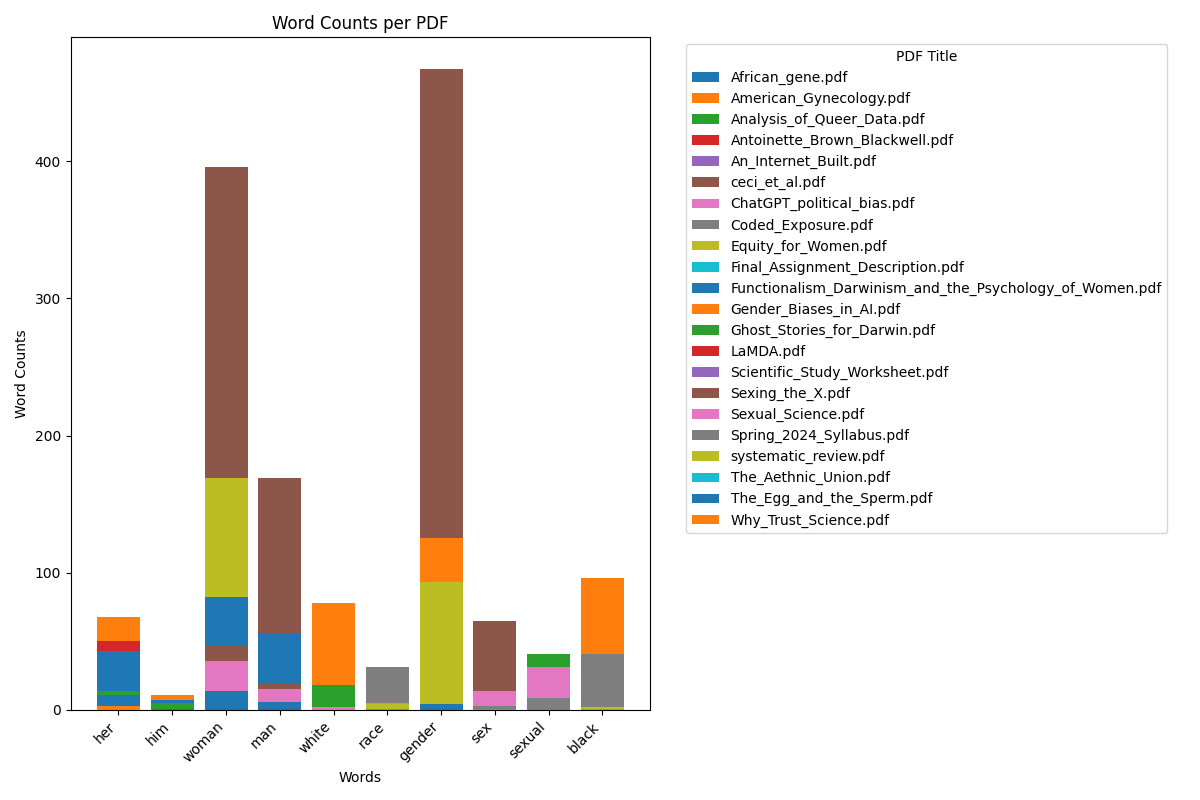
\includegraphics[width=\textwidth]{word counts.png}

\end{document}